\documentclass[11pt,aspectratio=169]{beamer}

% Packages
% Shared content style for NN and NNDS. Written by Claude (2026-10-14).
%
% Everything that shared slides rely on lives here, loaded by both courses:
% colors, notation helpers and the card system. Course themes own only the
% presentation around the content (header, footer, title page, fonts, the
% \myalert color and where \SlideSource text goes). Change a definition here,
% never by redefining it in a course file, so the two courses cannot drift.

\usepackage{mathtools,amssymb,tcolorbox}
\tcbsetforeverylayer{autoparskip}

% Semantic colors
\definecolor{darkred}{rgb}{0.55,0,0}
\definecolor{darkpastelblue}{rgb}{0.47,0.62,0.8}
\definecolor{darkcerulean}{rgb}{0.03,0.27,0.49}
\definecolor{darkgreen}{rgb}{0,0.55,0}

% Figure palette (draw.io defaults)
\definecolor{titlecolor}{RGB}{245, 242, 238}
\definecolor{drawgray}{HTML}{666666}
\definecolor{drawgray_l}{HTML}{F5F5F5}
\definecolor{drawblue}{HTML}{6C8EBF}
\definecolor{drawblue_l}{HTML}{DAE8FC}
\definecolor{drawgreen}{HTML}{82B366}
\definecolor{drawgreen_l}{HTML}{D5E8D4}
\definecolor{draworange}{HTML}{D79B00}
\definecolor{draworange_l}{HTML}{FFE6CC}
\definecolor{drawyellow}{HTML}{D6B656}
\definecolor{drawyellow_l}{HTML}{FFF2CC}
\definecolor{drawred}{HTML}{B85450}
\definecolor{drawred_l}{HTML}{EA6B66}
\definecolor{drawviolet}{HTML}{9673A6}
\definecolor{drawviolet_l}{HTML}{E1D5E7}

% Notation
\newcommand{\vc}[1]{\boldsymbol{\mathbf{#1}}}
\DeclareMathOperator*{\argmax}{arg\,max}
\DeclareMathOperator*{\argmin}{arg\,min}

% Cards: blue for definitions and computable quantities, green for goals and
% stable formulations, orange for warnings and trade-offs, red for
% training-specific or problematic elements.
\tcbset{
	nndsblue/.style={colback=drawblue_l!35!white,colframe=drawblue,boxrule=0.8pt,arc=1mm},
	nndsgreen/.style={colback=drawgreen_l!35!white,colframe=drawgreen,boxrule=0.8pt,arc=1mm},
	nndsorange/.style={colback=draworange_l!35!white,colframe=draworange,boxrule=0.8pt,arc=1mm},
	nndsred/.style={colback=drawred_l!12!white,colframe=drawred,boxrule=0.8pt,arc=1mm}
}

% A card that opens with \[ would start with an empty paragraph line plus the
% display skip, leaving more room above than below (by an amount that differs
% between engines). Set that leading equation as a centered display-style line
% instead, so the space above it is the card padding, as below.
\makeatletter
\newcommand{\nndscardlead}{\futurelet\nndscard@next\nndscard@check}
% tcolorbox follows this hook with \ignorespaces; look past it.
\def\nndscard@check{\ifx\nndscard@next\ignorespaces
	\expandafter\nndscard@skip\else\expandafter\nndscard@test\fi}
\def\nndscard@skip\ignorespaces{\nndscard@test}
\newcommand{\nndscard@test}{\@ifnextchar\[{\nndscard@display}{}}
\def\nndscard@display\[#1\]{{\centering$\displaystyle#1$\par}\@ifnextchar\end{}{\vspace{\belowdisplayskip}}}
\makeatother

% Card text is ragged-right: narrow justified columns open wide word gaps,
% especially in NNDS, which never hyphenates. Fixed display spacing: when
% parallel cards share a height, stretchable skips would otherwise spread
% the content unevenly.
\tcbset{
	nndscard/.style={before upper={\raggedright
		\setlength{\abovedisplayskip}{6pt}\setlength{\belowdisplayskip}{6pt}%
		\setlength{\abovedisplayshortskip}{6pt}\setlength{\belowdisplayshortskip}{6pt}%
		\nndscardlead}},
	nndsblue/.append style={nndscard},
	nndsgreen/.append style={nndscard},
	nndsorange/.append style={nndscard},
	nndsred/.append style={nndscard}
}

% Parallel cards share a group name and get equal heights; the second argument
% (a fixed height used by older NNDS slides) is ignored.
\tcbset{courseheight/.style 2 args={equal height group=#1}}

\usepackage{mathtools}
\usepackage{hyperref}
\usepackage{setspace}
\usepackage{tikz}
\usetikzlibrary{positioning}
\usepackage{ragged2e}
\usepackage{nicematrix}
\usepackage[compatibility=false]{caption}
\usepackage[framemethod=tikz]{mdframed}


% Theme
\usetheme{metropolis}
\metroset{subsectionpage=progressbar,sectionpage=none}
\setbeamertemplate{theorems}[numbered]

\usepackage{fontspec}
\defaultfontfeatures{LetterSpace=30}
\usepackage{microtype}

% Prefer flexible inter-word spacing over splitting words across lines.
\tolerance=1
\emergencystretch=\maxdimen
\hyphenpenalty=10000
\hbadness=10000


% Code
\usepackage{listings}
% Custom colors
\definecolor{codegreen}{rgb}{0,0.6,0}
\definecolor{codegray}{rgb}{0.5,0.5,0.5}
\definecolor{codepurple}{rgb}{0.58,0,0.82}
\definecolor{backcolour}{rgb}{0.95,0.95,0.92}
\definecolor{light-gray}{gray}{0.95}
% Python style for highlighting
\newcommand\pythonstyle{\lstset{
		backgroundcolor=\color{white},
		language=Python,
		basicstyle=\ttfamily\footnotesize,
		morekeywords={self},              % Add keywords here
		keywordstyle=\color{blue},
		stringstyle=\footnotesize\color{deepgreen},
		commentstyle=\color{codegreen},
		showstringspaces=false,
		frame=tb,
		numbers=left,
		numbersep=5pt,
		numberstyle=\tiny\color{gray},
		columns=fullflexible,
		numbersep=5pt,
		aboveskip=1em,
		showtabs=false,
		tabsize=2,
		gobble=3
	}}

% Python environment
\lstnewenvironment{python}[1][]
{
	\pythonstyle
	\lstset{#1}
}
{}
% Python for inline
\newcommand\pythoninline[1]{{\pythonstyle\lstinline!#1!}}

% Tables and justification
\newcommand{\ra}[1]{\renewcommand{\arraystretch}{#1}}
\justifying

% Subfigures
\setbeamertemplate{caption}[numbered]
\usepackage[caption=false,font=footnotesize]{subfig}

% Colors
\setbeamercolor{uppercolgreen}{fg=white,bg=green!35}
\setbeamercolor{lowercolgreen}{fg=black,bg=green!10}
\setbeamercolor{uppercolred}{fg=white,bg=red!35}
\setbeamercolor{lowercolred}{fg=black,bg=red!10}
\setbeamercolor{uppercolblue}{fg=white,bg=blue!35}
\setbeamercolor{lowercolblue}{fg=black,bg=blue!10}
\definecolor{deepblue}{rgb}{0,0,0.5}
\definecolor{deepred}{rgb}{0.6,0,0}
\definecolor{deepgreen}{rgb}{0,0.5,0}

% Matrix size
\usepackage{stackengine}
\stackMath
\def\sss{\scriptstyle \color{gray}}
\setstackgap{L}{12pt}
\def\stacktype{L}

% Mathematical commands
\newcommand{\pr}[1]{{#1\,}'}
\newcommand{\idx}[2]{{\color{darkpastelblue}[}#1{\color{darkpastelblue}]_{#2}}}
\newcommand{\shape}[2]{\stackunder{#1}{\sss #2}}

% Style commands
\newcommand{\myalert}[1]{{\color{darkred}\textbf{#1}}}

% White background on every slide, so figures with a white canvas blend in
% (Simone, 2026-10-14). whiteframe is kept as an alias for existing slides.
\setbeamercolor{background canvas}{bg=white}

% White frame (for images)
\newenvironment{whiteframe}[1]{
	\setbeamercolor{background canvas}{bg=white}
	\begin{frame}{#1}
		}{
	\end{frame}
}

\setbeamerfont{frametitle}{size=\normalsize}
\setbeamertemplate{frametitle}[default][right]
% Slimmer header, close to NN's share of the slide height (Simone, 2026-10-14).
\makeatletter
\patchcmd{\beamer@@tmpl@frametitle}{sep=0.3cm}{sep=0.2cm}{}{\PackageWarning{style}{frametitle padding not patched}}
\makeatother
{
}
%\setbeamercolor{frametitle}{fg=white,bg=black!75}

% No headline frame
\makeatletter
\newenvironment{noheadline}{
	\setbeamertemplate{headline}{}
	\addtobeamertemplate{frametitle}{\vspace*{-3.5\baselineskip}}{}
}{}
\makeatother

% Lists
\setbeamertemplate{itemize items}[triangle]

% Footnotes
\setbeamertemplate{footnote}%
{%
	\parindent 1.5em\noindent%
	\justifying\setstretch{0.7}%
	\hbox to 1em{\hfil\insertfootnotemark}\begin{scriptsize}\insertfootnotetext\end{scriptsize}\par%
}

% Footnote without number
\newcommand\blfootnote[1]{%
	\begingroup
	\renewcommand\thefootnote{}\footnote[frame]{\noindent#1}%
	\addtocounter{footnote}{-1}%
	\endgroup
}

% Slide sources: set in the frame footer beside the page number, so they
% take no room from the content. Zero height keeps the footline unchanged.
% Global, because the footline is typeset outside the frame's group; each
% frame starts empty.
\newcommand{\insertslidesource}{}
\newcommand{\SlideSource}[1]{\gdef\insertslidesource{#1}}
\AddToHook{env/frame/begin}{\gdef\insertslidesource{}}
\setbeamertemplate{frame footer}{%
	\ifx\insertslidesource\empty\else
		\smash{\parbox[b]{0.88\textwidth}{\raggedright\scriptsize\color{black!60}\insertslidesource}}%
	\fi}

% Theorems
\newcommand*{\theorembreak}{\usebeamertemplate{theorem end}\framebreak\usebeamertemplate{theorem begin}}
\newcounter{theo}[section]\setcounter{theo}{0}
\renewcommand{\thetheo}{\arabic{section}.\arabic{theo}}

\newenvironment{theo}[2][]{%
	\refstepcounter{theo}%
	\ifstrempty{#1}%
	{\mdfsetup{%
			frametitle={%
					\tikz[baseline=(current bounding box.east),outer sep=0pt]
					\node[anchor=east,rectangle,fill=red!10]
					{\strut Theorem~\thetheo};}}
	}%
	{\mdfsetup{%
			frametitle={%
					\tikz[baseline=(current bounding box.east),outer sep=0pt]
					\node[anchor=east,rectangle,fill=red!10]
					{\strut Theorem~\thetheo:~#1};}}%
	}%
	\mdfsetup{innertopmargin=5pt,linecolor=red!10,%
		linewidth=2pt,topline=true,%
		frametitleaboveskip=\dimexpr-\ht\strutbox\relax
	}
	\begin{mdframed}[]\relax%
		\label{#2}}{\end{mdframed}}

\usetikzlibrary{arrows.meta,calc}
\usepackage{pgfplots}
\pgfplotsset{compat=1.18}
\usepgfplotslibrary{groupplots}
\graphicspath{{assets/}{../../shared/assets/}}

% Draft by Claude (2026-10-20): refresh of the 2024 "Building deep networks"
% deck. Table of contents agreed in the Courses side conversation; this file
% starts with the opening section.

\begin{document}

{\usebackgroundtemplate{\tikz\node[opacity=0.4,inner sep=0]{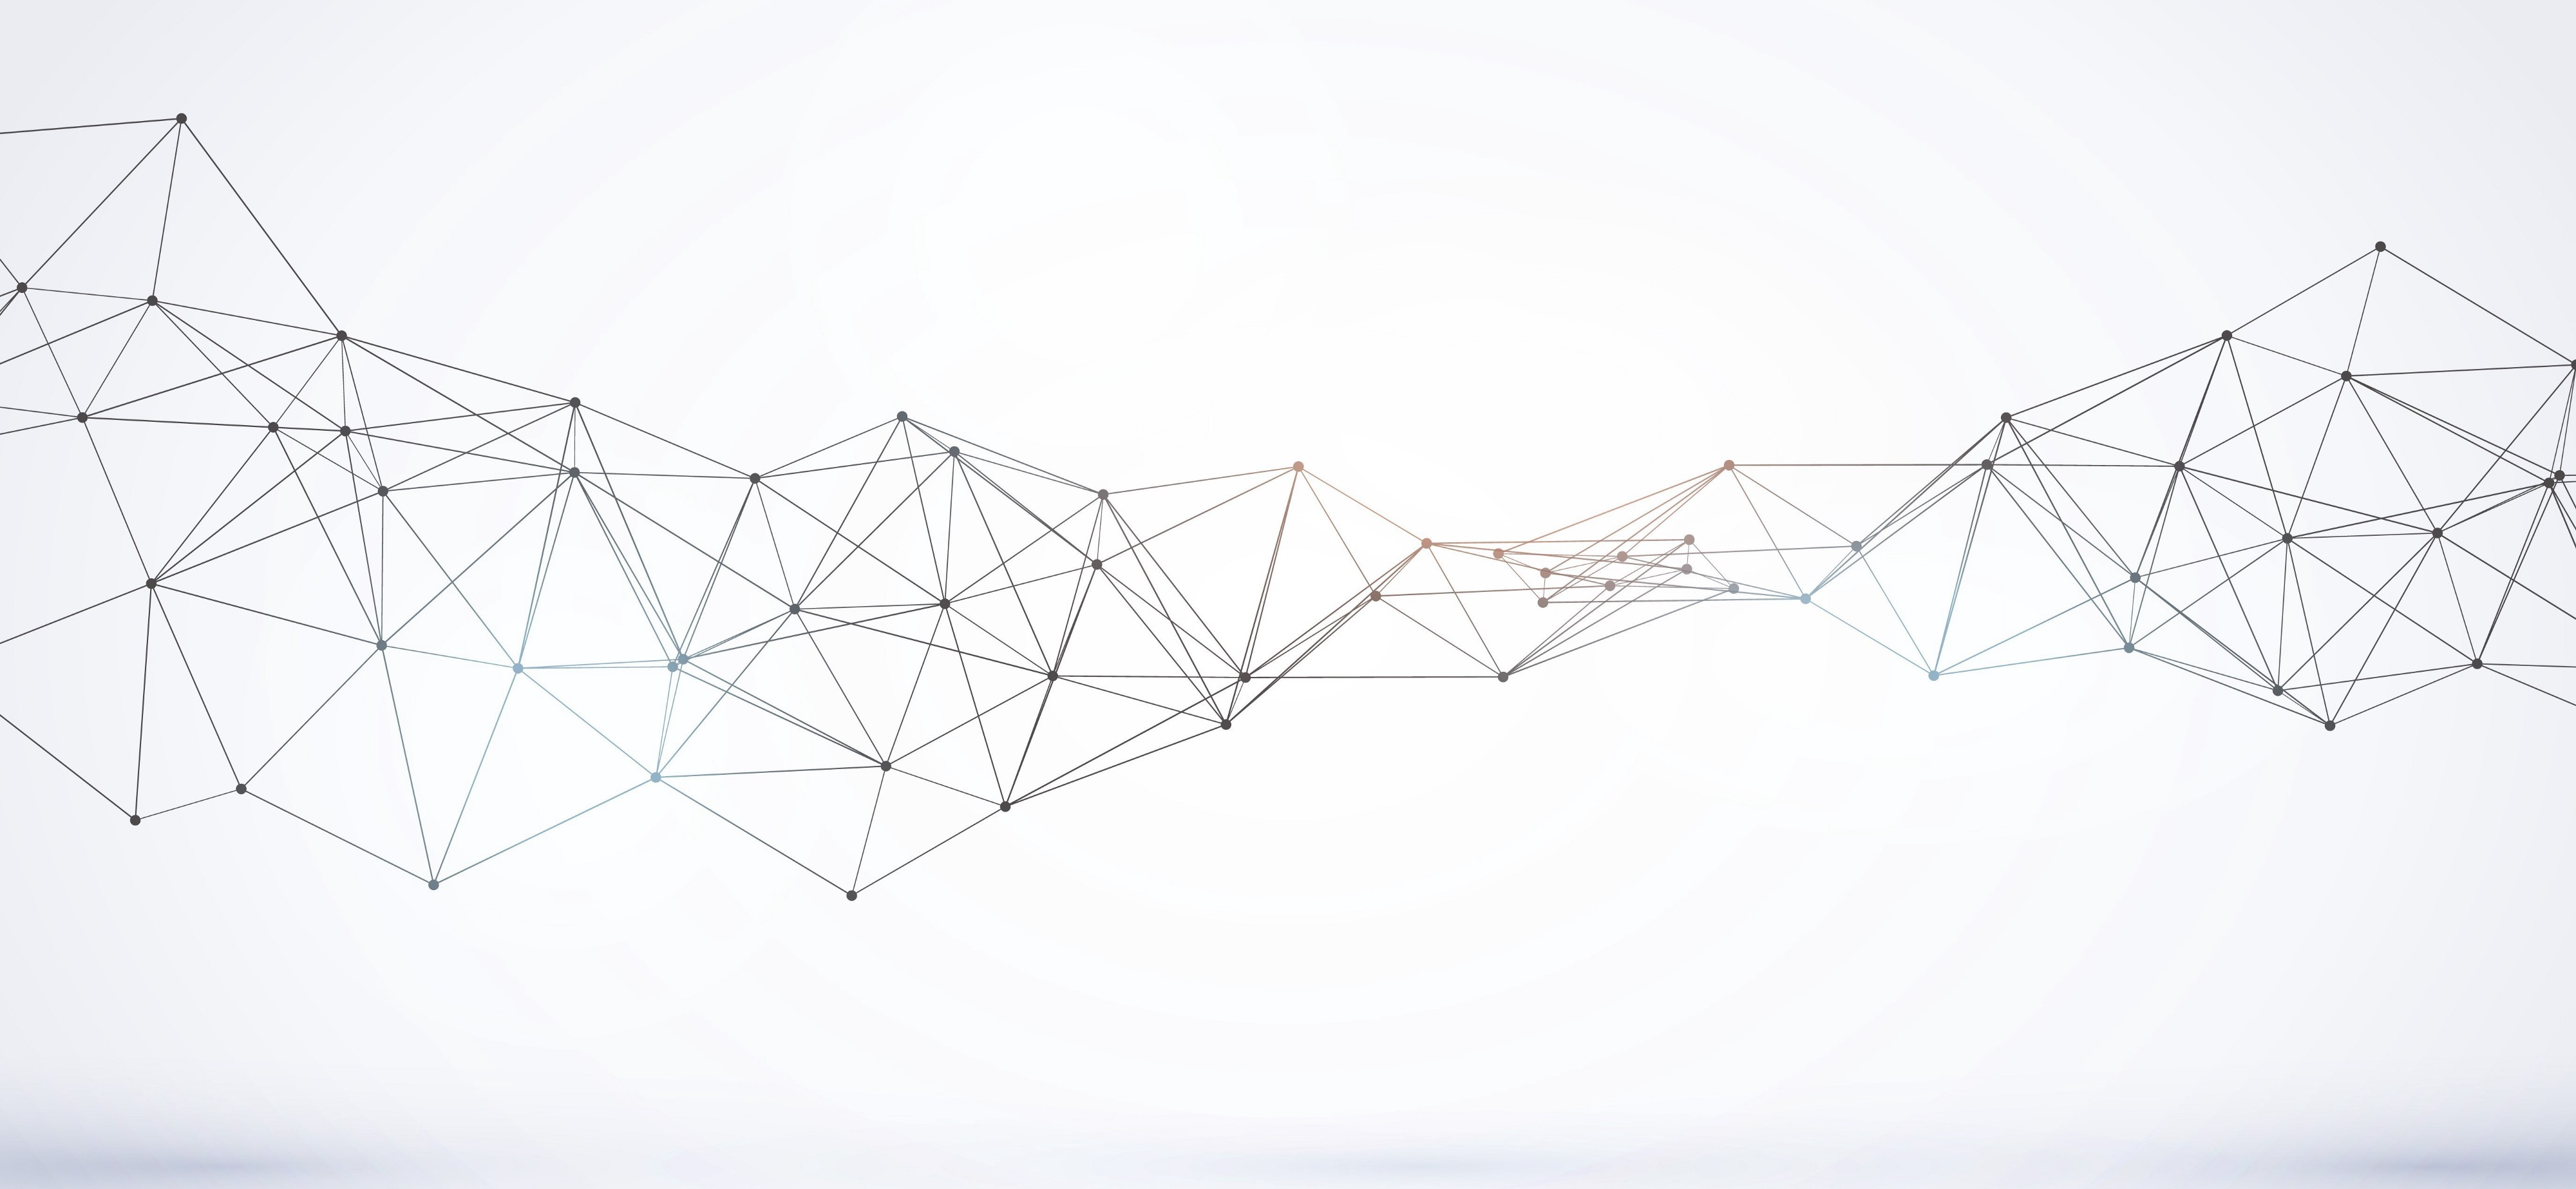
\includegraphics[width=\paperwidth,height=\paperheight]{images/header}};}%
\begin{frame}[plain]
    \vspace{0.5cm}
    \title{\large \begin{spacing}{1.0}Neural Networks for Data Science\end{spacing}\vspace{0.25em}
        \normalsize \begin{spacing}{1.0}\textbf{Master's Degree in Data Science}\end{spacing}\vspace{0.5em}}
    \subtitle{\Large \textbf{Building deeper models}}
    \date{
        {
\includegraphics[scale=0.8]{images/Uniroma1}}
    }
    \author{
        \setlength{\tabcolsep}{2pt}
        \begin{tabular}{rl}
            \textbf{Lecturer}: & S. Scardapane \\
        \end{tabular}
    }\titlepage
\end{frame}
}

\section{Why depth is hard}
\subsection{Going deeper}

% Figures from Russakovsky et al. (2015), IJCV: Sec. 2 (21,841 synsets,
% 14,197,122 images as of August 2014), Table 2 (ILSVRC2012 split), Sec. 4.1
% (top-5 metric, 120 dog breeds).
\begin{frame}{ImageNet and its challenge}

    \begin{columns}[T,onlytextwidth]
        \begin{column}{0.48\textwidth}
            \begin{tcolorbox}[nndsblue,courseheight={imagenet}{}]
                \textbf{ImageNet (2009)}

                About 14 million images, labelled into some 22,000
                categories of the WordNet hierarchy.
            \end{tcolorbox}
        \end{column}
        \begin{column}{0.48\textwidth}
            \begin{tcolorbox}[nndsblue,courseheight={imagenet}{}]
                \textbf{ILSVRC (2010-2017)}

                A yearly competition on a subset: 1,000 classes, 1.28 million
                training and 50,000 validation images.
            \end{tcolorbox}
        \end{column}
    \end{columns}

    \medskip
    \begin{tcolorbox}[nndsblue]
        The \textbf{top-5 error} is the fraction of test images whose true
        class is not among the five classes with the highest score.
    \end{tcolorbox}

    \medskip
    Why five guesses? An image often contains several objects but has a
    single label, and some classes are very close: there are 120 dog breeds
    alone.

    \SlideSource{Deng et al. (2009), CVPR; Russakovsky et al. (2015), IJCV.}

\end{frame}

% Depth and top-5 error: ILSVRC table in Szegedy et al. (2015), Table 2
% (no external data), He et al. (2016) abstract. Tricks: Krizhevsky et al.
% (2012); Simonyan and Zisserman (2015), Sec. 3.1 (initialising deeper nets
% from net A); Szegedy et al. (2015), Sec. 5 (auxiliary classifiers "increase
% the gradient signal"); He et al. (2015); Ioffe and Szegedy (2015); Srivastava
% et al. (2015).
\begin{frame}{Going deeper on ImageNet}

    \begin{columns}[c,onlytextwidth]
        \begin{column}{0.47\textwidth}
            \centering
            \begin{tikzpicture}
                \begin{axis}[
                        width=\linewidth, height=0.6\textheight,
                        ymode=log, ymin=4, ymax=300,
                        xmin=2011.5, xmax=2015.6,
                        xtick={2012,2013,2014,2015}, xticklabel style={/pgf/number format/1000 sep={}},
                        ytick={8,20,50,150}, yticklabels={8,20,50,150},
                        ylabel={Layers}, ylabel style={font=\small},
                        tick label style={font=\small},
                        axis lines=left, axis line style={drawgray},
                        clip=false,
                    ]
                    \addplot[draworange!70, dashed, thin]
                    coordinates {(2012,8) (2013,8) (2014.08,22) (2015,152)};
                    \addplot[draworange, mark=*, mark size=2.2pt, only marks]
                    coordinates {(2012,8) (2013,8) (2013.92,19) (2014.08,22) (2015,152)};
                    \node[font=\scriptsize, anchor=south, align=center] at (axis cs:2012,9) {AlexNet\\16.4\%};
                    \node[font=\scriptsize, anchor=south, align=center] at (axis cs:2013,9) {ZFNet\\11.7\%};
                    \node[font=\scriptsize, anchor=north, align=center] at (axis cs:2013.92,16.5) {VGG\\7.3\%};
                    \node[font=\scriptsize, anchor=west, align=left] at (axis cs:2014.16,23) {GoogLeNet\\6.7\%};
                    \node[font=\scriptsize, anchor=east, align=right] at (axis cs:2014.92,152) {ResNet\\3.6\%};
                \end{axis}
            \end{tikzpicture}

            {\scriptsize ILSVRC winners (and VGG): depth and top-5 error.}
        \end{column}
        \begin{column}{0.49\textwidth}%
            \small%
            \setlength{\parskip}{4pt}%
            \RaggedRight\setlength{\parindent}{0pt}%
            Every jump in depth needed a new trick to keep training working.

            \textbf{2012} ReLU, dropout, data augmentation.

            \textbf{2014} Starting from a trained shallow network (VGG);
            extra classifiers halfway through the network (GoogLeNet).

            \textbf{2015} He initialization, \myalert{batch normalization},
            gated shortcuts, \myalert{residual connections}.

            \textbf{2016--17} Stochastic depth, dense connections (DenseNet),
            squeeze-and-excitation (SENet, the last winner: 2.3\%).
        \end{column}
    \end{columns}

    \medskip
    Not all tricks remain useful today, so we only cover the most important
    subset.

    \SlideSource{Szegedy et al. (2015), Table 2; Simonyan and Zisserman (2015);
        He et al. (2015); Ioffe and Szegedy (2015); Srivastava et al. (2015); He et al. (2016);
        Huang et al. (2016, 2017); Hu et al. (2018).}

\end{frame}

% LeNet/AlexNet figure from the 2024 deck (Dive into Deep Learning, Sec. 8.1,
% CC BY-SA 4.0). MNIST strip: assets/images/deeper/mnist_strip.py.
\begin{frame}{From LeNet to AlexNet}

    \begin{columns}[c,onlytextwidth]
        \begin{column}{0.42\textwidth}
            \centering
            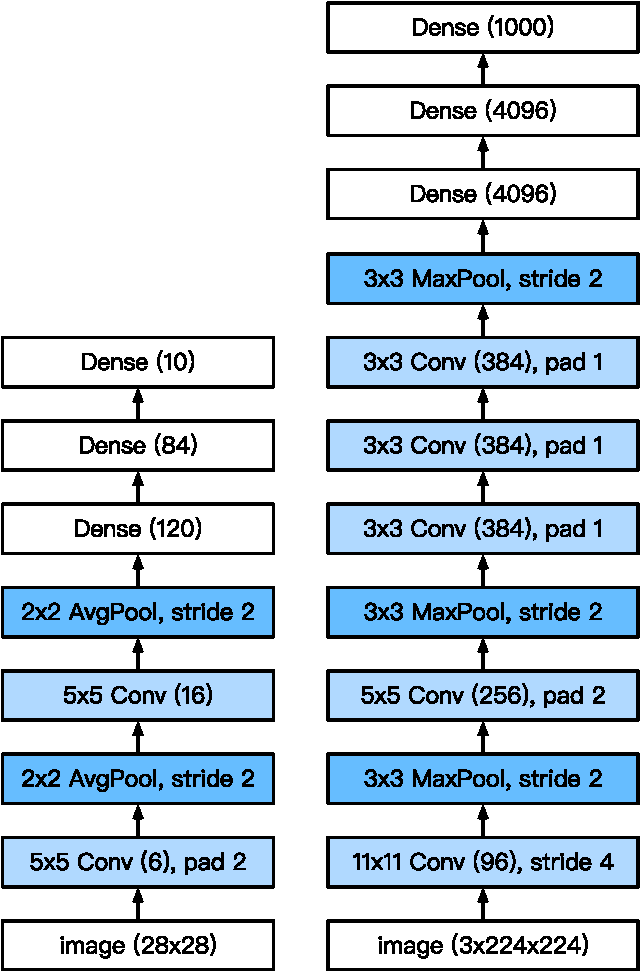
\includegraphics[height=0.76\textheight]{images/deeper/lenet_alexnet.pdf}

            {\scriptsize LeNet-5 (1998) and AlexNet (2012), simplified.}
        \end{column}
        \begin{column}{0.52\textwidth}%
            \setlength{\parskip}{6pt}%
            \RaggedRight\setlength{\parindent}{0pt}%
            In 1998, \myalert{LeNet-5} already read handwritten digits
            (\textbf{MNIST}) with convolutions, pooling and a small classifier.

            
\includegraphics[width=\linewidth]{images/deeper/mnist_strip.png}

            AlexNet is essentially a bigger LeNet! What changed in 2012 was
            GPUs, a large labelled dataset and a few training tricks.
        \end{column}
    \end{columns}

    \SlideSource{LeCun et al. (1998), Proc.\ IEEE; Krizhevsky et al. (2012), NeurIPS.
        Figure: Dive into Deep Learning, Sec.~8.1 (CC BY-SA 4.0).}

\end{frame}

% Opening experiment (Written by Claude, 2026-10-20). Data: opener.csv from
% assets/images/deeper/opener_table.py over depth_sweep.py runs (plain
% networks, 30 epochs, best of three learning rates per point, one seed).
\begin{frame}{Can we just stack more layers?}

    \begin{columns}[c,onlytextwidth]
        \begin{column}{0.36\textwidth}%
            \small\setlength{\parskip}{6pt}%
            \RaggedRight\setlength{\parindent}{0pt}%
            A plain CNN on \textbf{CIFAR-10} (60,000 small color images,
            10 classes): blocks of two $3\times3$ convolutions with ReLU, global
            pooling, a linear classifier.

            We change only the depth and the initialization, keeping the best
            of three learning rates.
        \end{column}
        \begin{column}{0.62\textwidth}
            \centering
            \begin{tikzpicture}
                \begin{groupplot}[
                        group style={group size=2 by 1, horizontal sep=1.1cm},
                        width=0.56\linewidth, height=0.46\textheight,
                        xmin=4, xmax=60, xtick={8,20,32,44,56},
                        tick label style={font=\scriptsize},
                        label style={font=\small}, title style={font=\small},
                        axis lines=left, axis line style={drawgray},
                        xlabel={Layers},
                        unbounded coords=jump,
                        every axis plot/.append style={thick, mark=*, mark size=1.6pt},
                    ]
                    \nextgroupplot[title={Training loss}, ymin=0, ymax=2.5]
                    \addplot[drawgray!60, dashed, thin, mark=none, forget plot] coordinates {(4,2.3026) (60,2.3026)};
                    \addplot[drawblue] table[x=depth, y=plain_he_loss, col sep=comma] {assets/images/deeper/opener.csv};
                    \addplot[draworange] table[x=depth, y=plain_default_loss, col sep=comma] {assets/images/deeper/opener.csv};
                    \node[font=\scriptsize, text=drawgray, anchor=north east] at (axis cs:59,2.25) {chance};
                    \nextgroupplot[title={Test accuracy (\%)}, ymin=0, ymax=100,
                        legend columns=2, legend style={font=\scriptsize, draw=none, fill=none,
                                at={(-0.2,-0.5)}, anchor=north, /tikz/every even column/.append style={column sep=8pt}}]
                    \addplot[drawgray!60, dashed, thin, mark=none, forget plot] coordinates {(4,10) (60,10)};
                    \addplot[drawblue] table[x=depth, y=plain_he_acc, col sep=comma] {assets/images/deeper/opener.csv};
                    \addplot[draworange] table[x=depth, y=plain_default_acc, col sep=comma] {assets/images/deeper/opener.csv};
                    \legend{He init, PyTorch default}
                \end{groupplot}
            \end{tikzpicture}
        \end{column}
    \end{columns}

    \medskip
    \begin{tcolorbox}[nndsorange]
        Deeper plain networks are worse on the \textbf{training} set, so this is
        not overfitting: we simply cannot optimize them.
    \end{tcolorbox}

    \SlideSource{Krizhevsky (2009), \textit{Learning multiple layers of features from tiny images}.}

\end{frame}

\begin{frame}{The rest of the lecture}
    \setlength{\parskip}{6pt}

    A good initialization (such as He's) only fixes the scale of the
    activations at the first step. Nothing keeps it there during training, and
    the gradient must cross every layer to reach the first ones.

    We look at three possible solutions to improve training at scale:

    \begin{columns}[T,onlytextwidth]
        \begin{column}{0.32\textwidth}
            \begin{tcolorbox}[nndsblue,courseheight={roadmap}{}]
                \textbf{Normalization}

                Keep the scale of the activations under control during training.
            \end{tcolorbox}
        \end{column}
        \begin{column}{0.32\textwidth}
            \begin{tcolorbox}[nndsred,courseheight={roadmap}{}]
                \textbf{Residuals}

                Make the identity the default, so every block only adds a small change.
            \end{tcolorbox}
        \end{column}
        \begin{column}{0.32\textwidth}
            \begin{tcolorbox}[nndsgreen,courseheight={roadmap}{}]
                \textbf{Regularization}

                Once the network trains, make it generalize.
            \end{tcolorbox}
        \end{column}
    \end{columns}

\end{frame}

\section{Normalization}
\subsection{Normalization layers}

% Written by Claude (2026-10-20). Fixes the 2024 slide: column index in the
% statistics, and "Hessian of X" (the Hessian is that of the least-squares loss).
\begin{frame}{Normalizing the inputs}
    \setlength{\parskip}{6pt}

    Given a dataset $\vc{X}\sim(N,D)$, we usually standardize each column
    (feature) to zero mean and unit variance:
    \[
        \idx{\vc{X}'}{i,j} = \frac{\idx{\vc{X}}{i,j} - \mu_j}{\sigma_j} \,, \qquad
        \mu_j = \frac{1}{N}\sum_i \idx{\vc{X}}{i,j} \,, \quad
        \sigma_j^2 = \frac{1}{N}\sum_i \left(\idx{\vc{X}}{i,j} - \mu_j\right)^2 .
    \]
    For least squares, the Hessian of the loss is $\frac{2}{N}\vc{X}^\top\vc{X}$.
    After standardization its diagonal is constant, so the problem is usually
    better \textbf{conditioned}: remember the elongated valley in the
    preliminaries.

    \begin{tcolorbox}[nndsgreen]
        Idea: do the same inside the network, on the output of every layer.
        The difficulty is that these outputs change at every step of training.
    \end{tcolorbox}

\end{frame}

\begin{frame}{Batch normalization}
    \setlength{\parskip}{5pt}

    Take the outputs of a layer on a mini-batch, $\vc{H}\sim(B,D)$. We
    estimate the statistics of each column on the mini-batch, and standardize:
    \[
        \widetilde{\mu}_j = \frac{1}{B}\sum_i \idx{\vc{H}}{i,j} \,, \quad
        \widetilde{\sigma}_j^2 = \frac{1}{B}\sum_i \left(\idx{\vc{H}}{i,j} - \widetilde{\mu}_j\right)^2 , \quad
        \idx{\vc{H}'}{i,j} = \frac{\idx{\vc{H}}{i,j} - \widetilde{\mu}_j}{\sqrt{\widetilde{\sigma}_j^2 + \varepsilon}} \,.
    \]
    A \myalert{batch normalization} (BN) layer then sets a new mean and scale
    for each column, with $2D$ trainable parameters:
    \[
        \idx{\text{BN}(\vc{H})}{i,j} = \gamma_j \idx{\vc{H}'}{i,j} + \beta_j \,.
    \]
    It usually goes between a linear (or convolutional) layer and its
    activation, whose bias becomes redundant.

    \SlideSource{Ioffe and Szegedy (2015), \textit{Batch normalization: accelerating deep network training by reducing internal covariate shift}, ICML.}

\end{frame}

\begin{frame}{Batch normalization at inference}
    \setlength{\parskip}{6pt}

    During training, the output for one example depends on the other examples
    in its mini-batch. At inference we want a deterministic prediction, even for
    a single input.

    During training, BN keeps a running average of the mini-batch statistics,
    for example
    \[
        \mu_j \leftarrow (1-m)\,\mu_j + m\,\widetilde{\mu}_j \,, \qquad m = 0.1 \,,
    \]
    and the same for the variance. At inference, it uses $\mu_j$ and
    $\sigma_j^2$ in place of $\widetilde{\mu}_j$ and $\widetilde{\sigma}_j^2$.

    \begin{tcolorbox}[nndsorange]
        The same layer behaves differently in training and inference. In
        PyTorch, \texttt{model.train()} and \texttt{model.eval()} switch between
        the two modes: forgetting \texttt{model.eval()} is a classic bug.
    \end{tcolorbox}

    \SlideSource{Wu and Johnson (2021), \textit{Rethinking ``batch'' in BatchNorm}.}

\end{frame}

% Figure: S. Scardapane, Alice's Adventures in a Differentiable Wonderland.
\begin{frame}{Which axes do we normalize?}

    \begin{columns}[c,onlytextwidth]
        \begin{column}{0.46\textwidth}
            \centering
            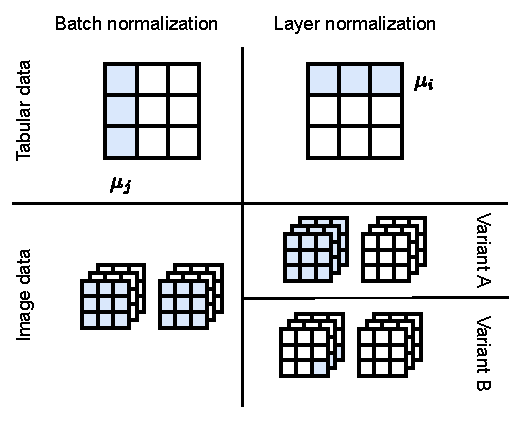
\includegraphics[width=\linewidth]{images/deeper/normalization_axes.pdf}
        \end{column}
        \begin{column}{0.5\textwidth}%
            \small\setlength{\parskip}{6pt}%
            \RaggedRight\setlength{\parindent}{0pt}%
            The statistics (blue) can be computed along different axes.

            \textbf{Batch normalization} averages over the mini-batch: one mean
            per feature, or per channel for images $(B,H,W,C)$.

            \myalert{Layer normalization} (LN) averages over the features of each
            example, independently of the others. For images, either over the
            whole image (variant A) or over the channels at each pixel
            (variant B).

            The parameters $\gamma, \beta$ have one entry per normalized
            feature or channel.
        \end{column}
    \end{columns}

    \SlideSource{Ba et al. (2016), \textit{Layer normalization}; Wu and He (2018), \textit{Group normalization}, ECCV.}

\end{frame}

\begin{frame}{From batch to layer normalization}
    \setlength{\parskip}{6pt}

    Batch normalization works very well for CNNs, but tying each example to its
    mini-batch has a cost:
    \begin{itemize}
        \item noisy estimates with small mini-batches;
        \item a poor fit for sequences of different lengths, or for training
              split across many devices;
        \item different behavior in training and inference.
    \end{itemize}
    Layer normalization avoids all three: it is the standard in transformers. Most recent LLMs use an even simpler variant, \myalert{RMSNorm},
    which skips the mean and only rescales each vector:
    \[
        \text{RMSNorm}(\vc{h}) = \vc{\gamma} \odot \frac{\vc{h}}{\sqrt{\frac{1}{D}\sum_j h_j^2 + \varepsilon}} \,.
    \]

    \SlideSource{Zhang and Sennrich (2019), \textit{Root mean square layer normalization}, NeurIPS.}

\end{frame}

\subsection{Why normalization works}

\begin{frame}{Why does normalization help?}
    \setlength{\parskip}{6pt}

    The original explanation was \textbf{internal covariate shift}: each layer
    sees inputs whose distribution keeps changing as the previous layers train,
    and BN would stabilize them.

    Later experiments do not support it: injecting noise after BN to shift the
    distributions again barely hurts training. A better-supported view is that
    BN makes the loss landscape \textbf{smoother}, so the gradient stays
    predictive over longer steps.

    \begin{tcolorbox}[nndsgreen]
        In practice, the most robust effect is that normalized networks train
        stably with much \textbf{larger learning rates}.
    \end{tcolorbox}

    The full picture is still debated: methods often work long before we
    understand why.

    \SlideSource{Santurkar et al. (2018), \textit{How does batch normalization help optimization?}, NeurIPS;
        Bjorck et al. (2018), \textit{Understanding batch normalization}, NeurIPS.}

\end{frame}

\begin{frame}{Normalized layers ignore the scale of their weights}
    \setlength{\parskip}{6pt}

    If a unit with weights $\vc{w}$ is followed by normalization, scaling
    $\vc{w}$ by any $a > 0$ changes nothing:
    \[
        \text{BN}(a\,\vc{X}\vc{w}) = \text{BN}(\vc{X}\vc{w}) \,.
    \]
    Only the direction of $\vc{w}$ matters. Two consequences for gradient descent:
    \begin{itemize}
        \item the gradient is orthogonal to $\vc{w}$, so plain steps can only
              make $\lVert\vc{w}\rVert$ grow;
        \item the gradient shrinks as $1/\lVert\vc{w}\rVert$, so the effective
              step on the direction is about $\eta / \lVert\vc{w}\rVert^2$.
    \end{itemize}

    \begin{tcolorbox}[nndsorange]
        For these weights, weight decay does not regularize the function: by keeping
        $\lVert\vc{w}\rVert$ small, it sets the \textbf{effective learning rate}.
    \end{tcolorbox}

    \SlideSource{van Laarhoven (2017), \textit{L2 regularization versus batch and weight normalization}.}

\end{frame}

\end{document}
